\PassOptionsToPackage{unicode=true}{hyperref} % options for packages loaded elsewhere
\PassOptionsToPackage{hyphens}{url}
%
\documentclass[]{article}
\usepackage{lmodern}
\usepackage{amssymb,amsmath}
\usepackage{ifxetex,ifluatex}
\usepackage{fixltx2e} % provides \textsubscript
\ifnum 0\ifxetex 1\fi\ifluatex 1\fi=0 % if pdftex
  \usepackage[T1]{fontenc}
  \usepackage[utf8]{inputenc}
  \usepackage{textcomp} % provides euro and other symbols
\else % if luatex or xelatex
  \usepackage{unicode-math}
  \defaultfontfeatures{Ligatures=TeX,Scale=MatchLowercase}
\fi
% use upquote if available, for straight quotes in verbatim environments
\IfFileExists{upquote.sty}{\usepackage{upquote}}{}
% use microtype if available
\IfFileExists{microtype.sty}{%
\usepackage[]{microtype}
\UseMicrotypeSet[protrusion]{basicmath} % disable protrusion for tt fonts
}{}
\IfFileExists{parskip.sty}{%
\usepackage{parskip}
}{% else
\setlength{\parindent}{0pt}
\setlength{\parskip}{6pt plus 2pt minus 1pt}
}
\usepackage{hyperref}
\hypersetup{
            pdftitle={R Notebook},
            pdfborder={0 0 0},
            breaklinks=true}
\urlstyle{same}  % don't use monospace font for urls
\usepackage[margin=1in]{geometry}
\usepackage{color}
\usepackage{fancyvrb}
\newcommand{\VerbBar}{|}
\newcommand{\VERB}{\Verb[commandchars=\\\{\}]}
\DefineVerbatimEnvironment{Highlighting}{Verbatim}{commandchars=\\\{\}}
% Add ',fontsize=\small' for more characters per line
\usepackage{framed}
\definecolor{shadecolor}{RGB}{248,248,248}
\newenvironment{Shaded}{\begin{snugshade}}{\end{snugshade}}
\newcommand{\AlertTok}[1]{\textcolor[rgb]{0.94,0.16,0.16}{#1}}
\newcommand{\AnnotationTok}[1]{\textcolor[rgb]{0.56,0.35,0.01}{\textbf{\textit{#1}}}}
\newcommand{\AttributeTok}[1]{\textcolor[rgb]{0.77,0.63,0.00}{#1}}
\newcommand{\BaseNTok}[1]{\textcolor[rgb]{0.00,0.00,0.81}{#1}}
\newcommand{\BuiltInTok}[1]{#1}
\newcommand{\CharTok}[1]{\textcolor[rgb]{0.31,0.60,0.02}{#1}}
\newcommand{\CommentTok}[1]{\textcolor[rgb]{0.56,0.35,0.01}{\textit{#1}}}
\newcommand{\CommentVarTok}[1]{\textcolor[rgb]{0.56,0.35,0.01}{\textbf{\textit{#1}}}}
\newcommand{\ConstantTok}[1]{\textcolor[rgb]{0.00,0.00,0.00}{#1}}
\newcommand{\ControlFlowTok}[1]{\textcolor[rgb]{0.13,0.29,0.53}{\textbf{#1}}}
\newcommand{\DataTypeTok}[1]{\textcolor[rgb]{0.13,0.29,0.53}{#1}}
\newcommand{\DecValTok}[1]{\textcolor[rgb]{0.00,0.00,0.81}{#1}}
\newcommand{\DocumentationTok}[1]{\textcolor[rgb]{0.56,0.35,0.01}{\textbf{\textit{#1}}}}
\newcommand{\ErrorTok}[1]{\textcolor[rgb]{0.64,0.00,0.00}{\textbf{#1}}}
\newcommand{\ExtensionTok}[1]{#1}
\newcommand{\FloatTok}[1]{\textcolor[rgb]{0.00,0.00,0.81}{#1}}
\newcommand{\FunctionTok}[1]{\textcolor[rgb]{0.00,0.00,0.00}{#1}}
\newcommand{\ImportTok}[1]{#1}
\newcommand{\InformationTok}[1]{\textcolor[rgb]{0.56,0.35,0.01}{\textbf{\textit{#1}}}}
\newcommand{\KeywordTok}[1]{\textcolor[rgb]{0.13,0.29,0.53}{\textbf{#1}}}
\newcommand{\NormalTok}[1]{#1}
\newcommand{\OperatorTok}[1]{\textcolor[rgb]{0.81,0.36,0.00}{\textbf{#1}}}
\newcommand{\OtherTok}[1]{\textcolor[rgb]{0.56,0.35,0.01}{#1}}
\newcommand{\PreprocessorTok}[1]{\textcolor[rgb]{0.56,0.35,0.01}{\textit{#1}}}
\newcommand{\RegionMarkerTok}[1]{#1}
\newcommand{\SpecialCharTok}[1]{\textcolor[rgb]{0.00,0.00,0.00}{#1}}
\newcommand{\SpecialStringTok}[1]{\textcolor[rgb]{0.31,0.60,0.02}{#1}}
\newcommand{\StringTok}[1]{\textcolor[rgb]{0.31,0.60,0.02}{#1}}
\newcommand{\VariableTok}[1]{\textcolor[rgb]{0.00,0.00,0.00}{#1}}
\newcommand{\VerbatimStringTok}[1]{\textcolor[rgb]{0.31,0.60,0.02}{#1}}
\newcommand{\WarningTok}[1]{\textcolor[rgb]{0.56,0.35,0.01}{\textbf{\textit{#1}}}}
\usepackage{graphicx,grffile}
\makeatletter
\def\maxwidth{\ifdim\Gin@nat@width>\linewidth\linewidth\else\Gin@nat@width\fi}
\def\maxheight{\ifdim\Gin@nat@height>\textheight\textheight\else\Gin@nat@height\fi}
\makeatother
% Scale images if necessary, so that they will not overflow the page
% margins by default, and it is still possible to overwrite the defaults
% using explicit options in \includegraphics[width, height, ...]{}
\setkeys{Gin}{width=\maxwidth,height=\maxheight,keepaspectratio}
\setlength{\emergencystretch}{3em}  % prevent overfull lines
\providecommand{\tightlist}{%
  \setlength{\itemsep}{0pt}\setlength{\parskip}{0pt}}
\setcounter{secnumdepth}{0}
% Redefines (sub)paragraphs to behave more like sections
\ifx\paragraph\undefined\else
\let\oldparagraph\paragraph
\renewcommand{\paragraph}[1]{\oldparagraph{#1}\mbox{}}
\fi
\ifx\subparagraph\undefined\else
\let\oldsubparagraph\subparagraph
\renewcommand{\subparagraph}[1]{\oldsubparagraph{#1}\mbox{}}
\fi

% set default figure placement to htbp
\makeatletter
\def\fps@figure{htbp}
\makeatother


\title{R Notebook}
\author{}
\date{\vspace{-2.5em}}

\begin{document}
\maketitle

This is an \href{http://rmarkdown.rstudio.com}{R Markdown} Notebook.
When you execute code within the notebook, the results appear beneath
the code.

Try executing this chunk by clicking the \emph{Run} button within the
chunk or by placing your cursor inside it and pressing
\emph{Cmd+Shift+Enter}.

Elle Reagan, epr427

\begin{Shaded}
\begin{Highlighting}[]
\CommentTok{#install.packages("mlbench")}
\CommentTok{#install.packages("lmtest")}
\KeywordTok{library}\NormalTok{(readxl)}
\KeywordTok{library}\NormalTok{(dplyr)}
\KeywordTok{library}\NormalTok{(tidyverse)}
\KeywordTok{library}\NormalTok{(ggplot2)}
\KeywordTok{library}\NormalTok{(lmtest)}
\CommentTok{#install.packages("sandwich")}
\KeywordTok{library}\NormalTok{(sandwich)}
\CommentTok{#install.packages("vegan")}
\KeywordTok{library}\NormalTok{(vegan)}
\CommentTok{#install.packages("readxl")}

\NormalTok{ Book4 <-}\StringTok{ }\KeywordTok{read_excel}\NormalTok{(}\StringTok{"cereal.xlsx"}\NormalTok{, }\DataTypeTok{skip =} \DecValTok{1}\NormalTok{)}
\NormalTok{cer<-}\StringTok{ }\NormalTok{Book4}

\NormalTok{cer1<-}\StringTok{ }\NormalTok{cer}\OperatorTok\KeywordTok{select}\NormalTok{(}\OperatorTok{-}\NormalTok{name)}
\NormalTok{cer1}\OperatorTok{$}\NormalTok{mfr<-}\KeywordTok{ifelse}\NormalTok{(cer}\OperatorTok{$}\NormalTok{mfr}\OperatorTok{==}\StringTok{ "K"}\NormalTok{, }\StringTok{"K"}\NormalTok{,}\StringTok{"N"}\NormalTok{)}
\KeywordTok{head}\NormalTok{(cer1)}
\end{Highlighting}
\end{Shaded}

\begin{verbatim}
## # A tibble: 6 x 5
##   mfr   calories sodium shelf  rating
##   <chr>    <dbl>  <dbl> <chr>   <dbl>
## 1 N           70    130 Top      68.4
## 2 N          120     15 Top      34.0
## 3 K           70    260 Top      59.4
## 4 K           50    140 Top      93.7
## 5 N          110    200 Top      34.4
## 6 N          110    180 Bottom   29.5
\end{verbatim}

\begin{Shaded}
\begin{Highlighting}[]
\NormalTok{cer}\OperatorTok{$}\NormalTok{mfr<-}\StringTok{ }\KeywordTok{ifelse}\NormalTok{(cer}\OperatorTok{$}\NormalTok{mfr}\OperatorTok{==}\StringTok{ "K"}\NormalTok{, }\DecValTok{1}\NormalTok{,}\DecValTok{0}\NormalTok{)}


\NormalTok{cer}\OperatorTok{$}\NormalTok{shelf <-}\StringTok{ }\KeywordTok{as.factor}\NormalTok{(cer}\OperatorTok{$}\NormalTok{shelf)}
\NormalTok{cer}\OperatorTok{$}\NormalTok{mfr<-}\StringTok{ }\KeywordTok{as.factor}\NormalTok{(cer}\OperatorTok{$}\NormalTok{mfr)}


\NormalTok{class_diag <-}\StringTok{ }\ControlFlowTok{function}\NormalTok{(probs,truth)\{}
\CommentTok{#CONFUSION MATRIX: CALCULATE ACCURACY, TPR, TNR, PPV}
\NormalTok{tab<-}\KeywordTok{table}\NormalTok{(}\KeywordTok{factor}\NormalTok{(probs}\OperatorTok{>}\NormalTok{.}\DecValTok{5}\NormalTok{,}\DataTypeTok{levels=}\KeywordTok{c}\NormalTok{(}\StringTok{"FALSE"}\NormalTok{,}\StringTok{"TRUE"}\NormalTok{)),truth)}
\NormalTok{acc=}\KeywordTok{sum}\NormalTok{(}\KeywordTok{diag}\NormalTok{(tab))}\OperatorTok{/}\KeywordTok{sum}\NormalTok{(tab)}
\NormalTok{sens=tab[}\DecValTok{2}\NormalTok{,}\DecValTok{2}\NormalTok{]}\OperatorTok{/}\KeywordTok{colSums}\NormalTok{(tab)[}\DecValTok{2}\NormalTok{]}
\NormalTok{spec=tab[}\DecValTok{1}\NormalTok{,}\DecValTok{1}\NormalTok{]}\OperatorTok{/}\KeywordTok{colSums}\NormalTok{(tab)[}\DecValTok{1}\NormalTok{]}
\NormalTok{ppv=tab[}\DecValTok{2}\NormalTok{,}\DecValTok{2}\NormalTok{]}\OperatorTok{/}\KeywordTok{rowSums}\NormalTok{(tab)[}\DecValTok{2}\NormalTok{]}
\ControlFlowTok{if}\NormalTok{(}\KeywordTok{is.numeric}\NormalTok{(truth)}\OperatorTok{==}\OtherTok{FALSE} \OperatorTok{&}\StringTok{ }\KeywordTok{is.logical}\NormalTok{(truth)}\OperatorTok{==}\OtherTok{FALSE}\NormalTok{) truth<-}\KeywordTok{as.numeric}\NormalTok{(truth)}\OperatorTok{-}\DecValTok{1}
\CommentTok{#CALCULATE EXACT AUC}
\NormalTok{ord<-}\KeywordTok{order}\NormalTok{(probs, }\DataTypeTok{decreasing=}\OtherTok{TRUE}\NormalTok{)}
\NormalTok{probs <-}\StringTok{ }\NormalTok{probs[ord]; truth <-}\StringTok{ }\NormalTok{truth[ord]}
\NormalTok{TPR=}\KeywordTok{cumsum}\NormalTok{(truth)}\OperatorTok{/}\KeywordTok{max}\NormalTok{(}\DecValTok{1}\NormalTok{,}\KeywordTok{sum}\NormalTok{(truth))}
\NormalTok{FPR=}\KeywordTok{cumsum}\NormalTok{(}\OperatorTok{!}\NormalTok{truth)}\OperatorTok{/}\KeywordTok{max}\NormalTok{(}\DecValTok{1}\NormalTok{,}\KeywordTok{sum}\NormalTok{(}\OperatorTok{!}\NormalTok{truth))}
\NormalTok{dup<-}\KeywordTok{c}\NormalTok{(probs[}\OperatorTok{-}\DecValTok{1}\NormalTok{]}\OperatorTok{>=}\NormalTok{probs[}\OperatorTok{-}\KeywordTok{length}\NormalTok{(probs)], }\OtherTok{FALSE}\NormalTok{)}
\NormalTok{TPR<-}\KeywordTok{c}\NormalTok{(}\DecValTok{0}\NormalTok{,TPR[}\OperatorTok{!}\NormalTok{dup],}\DecValTok{1}\NormalTok{); FPR<-}\KeywordTok{c}\NormalTok{(}\DecValTok{0}\NormalTok{,FPR[}\OperatorTok{!}\NormalTok{dup],}\DecValTok{1}\NormalTok{)}
\NormalTok{n <-}\StringTok{ }\KeywordTok{length}\NormalTok{(TPR)}
\NormalTok{auc<-}\StringTok{ }\KeywordTok{sum}\NormalTok{( ((TPR[}\OperatorTok{-}\DecValTok{1}\NormalTok{]}\OperatorTok{+}\NormalTok{TPR[}\OperatorTok{-}\NormalTok{n])}\OperatorTok{/}\DecValTok{2}\NormalTok{) }\OperatorTok{*}\StringTok{ }\NormalTok{(FPR[}\OperatorTok{-}\DecValTok{1}\NormalTok{]}\OperatorTok{-}\NormalTok{FPR[}\OperatorTok{-}\NormalTok{n]) )}
\KeywordTok{data.frame}\NormalTok{(acc,sens,spec,ppv,auc)}
\NormalTok{\}}
\end{Highlighting}
\end{Shaded}

\begin{Shaded}
\begin{Highlighting}[]
\CommentTok{#Question 0.}

\CommentTok{#My datset is a collection of cereals with their name, whether or not they were manufactured by Kellog's, calories per serving, sodium in mg, what shelf they are placed on, and overall rating. I got this dataset from Kaggle. In total, there are 77 observations. }
\end{Highlighting}
\end{Shaded}

\begin{Shaded}
\begin{Highlighting}[]
\CommentTok{#Question 1.}

\CommentTok{#MANOVA}
\NormalTok{man1<-}\KeywordTok{manova}\NormalTok{(}\KeywordTok{cbind}\NormalTok{(rating,sodium, calories )}\OperatorTok{~}\NormalTok{shelf, }\DataTypeTok{data=}\NormalTok{cer)}

\KeywordTok{summary}\NormalTok{(man1)}
\end{Highlighting}
\end{Shaded}

\begin{verbatim}
##           Df  Pillai approx F num Df den Df   Pr(>F)   
## shelf      2 0.24965   3.4706      6    146 0.003094 **
## Residuals 74                                           
## ---
## Signif. codes:  0 '***' 0.001 '**' 0.01 '*' 0.05 '.' 0.1 ' ' 1
\end{verbatim}

\begin{Shaded}
\begin{Highlighting}[]
\CommentTok{#we see that the pvalue is less than .05 and so we reject the null hypothesis and continue on to univariate ANOVA}

\CommentTok{#univariate ANOVA}
\KeywordTok{summary.aov}\NormalTok{(man1)}
\end{Highlighting}
\end{Shaded}

\begin{verbatim}
##  Response rating :
##             Df  Sum Sq Mean Sq F value  Pr(>F)  
## shelf        2  1719.8  859.92  4.7928 0.01103 *
## Residuals   74 13277.0  179.42                  
## ---
## Signif. codes:  0 '***' 0.001 '**' 0.01 '*' 0.05 '.' 0.1 ' ' 1
## 
##  Response sodium :
##             Df Sum Sq Mean Sq F value Pr(>F)
## shelf        2   9628  4814.1  0.6792 0.5101
## Residuals   74 524489  7087.7               
## 
##  Response calories :
##             Df  Sum Sq Mean Sq F value Pr(>F)
## shelf        2   559.5  279.74  0.7317 0.4845
## Residuals   74 28292.5  382.33
\end{verbatim}

\begin{Shaded}
\begin{Highlighting}[]
\CommentTok{#we see that for rating and sodium the shelf position differs whereas calories do not}

\NormalTok{diffmeans<-}\StringTok{ }\NormalTok{cer}\OperatorTok\KeywordTok{group_by}\NormalTok{(shelf)}\OperatorTok\KeywordTok{summarize}\NormalTok{(}\KeywordTok{mean}\NormalTok{(rating),}\KeywordTok{mean}\NormalTok{(sodium))}
\NormalTok{diffmeans}
\end{Highlighting}
\end{Shaded}

\begin{verbatim}
## # A tibble: 3 x 3
##   shelf  `mean(rating)` `mean(sodium)`
##   <fct>           <dbl>          <dbl>
## 1 Bottom           46.1           176.
## 2 Middle           35.0           146.
## 3 Top              45.2           159.
\end{verbatim}

\begin{Shaded}
\begin{Highlighting}[]
\CommentTok{#we see the difference in means in both groups}

\KeywordTok{pairwise.t.test}\NormalTok{(cer}\OperatorTok{$}\NormalTok{sodium,cer}\OperatorTok{$}\NormalTok{shelf,}
                \DataTypeTok{p.adj=}\StringTok{"none"}\NormalTok{)}
\end{Highlighting}
\end{Shaded}

\begin{verbatim}
## 
##  Pairwise comparisons using t tests with pooled SD 
## 
## data:  cer$sodium and cer$shelf 
## 
##        Bottom Middle
## Middle 0.25   -     
## Top    0.45   0.58  
## 
## P value adjustment method: none
\end{verbatim}

\begin{Shaded}
\begin{Highlighting}[]
\CommentTok{#we see that the middle and bottom and top and bottom are significant }
\KeywordTok{pairwise.t.test}\NormalTok{(cer}\OperatorTok{$}\NormalTok{rating,cer}\OperatorTok{$}\NormalTok{shelf,}
                \DataTypeTok{p.adj=}\StringTok{"none"}\NormalTok{)}
\end{Highlighting}
\end{Shaded}

\begin{verbatim}
## 
##  Pairwise comparisons using t tests with pooled SD 
## 
## data:  cer$rating and cer$shelf 
## 
##        Bottom Middle
## Middle 0.0093 -     
## Top    0.8050 0.0068
## 
## P value adjustment method: none
\end{verbatim}

\begin{Shaded}
\begin{Highlighting}[]
\CommentTok{#we see that the top and middle are significant}

\CommentTok{#number of tests: one manova, 3 anova and 6 t tests}
\FloatTok{.05}\OperatorTok{/}\DecValTok{10}
\end{Highlighting}
\end{Shaded}

\begin{verbatim}
## [1] 0.005
\end{verbatim}

\begin{Shaded}
\begin{Highlighting}[]
\CommentTok{#bonferonni is .005}
\CommentTok{#after bonferonni the bottom and middle and top and middle are significant for sugars but rating is no longer significant}

\CommentTok{#type one error}
\DecValTok{1}\OperatorTok{-}\NormalTok{(.}\DecValTok{95}\OperatorTok{^}\DecValTok{10}\NormalTok{)}
\end{Highlighting}
\end{Shaded}

\begin{verbatim}
## [1] 0.4012631
\end{verbatim}

\begin{Shaded}
\begin{Highlighting}[]
\CommentTok{#type 1 error is .4012631}
\end{Highlighting}
\end{Shaded}

I think that this data has passed assumptions for random samples and
independent observations. The data does not pass for multivariate
normality of DV's since each group does not have greater than 25 counts.
Based on this, it would be difficult for the data to pass other
assumptions because the dataset is very small.

\begin{Shaded}
\begin{Highlighting}[]
\CommentTok{#Question 2.}

\NormalTok{dists<-cer}\OperatorTok\KeywordTok{select}\NormalTok{(sodium, calories)}\OperatorTok\KeywordTok{dist}\NormalTok{()}
\KeywordTok{adonis}\NormalTok{(dists}\OperatorTok{~}\NormalTok{shelf,}\DataTypeTok{data=}\NormalTok{cer)}
\end{Highlighting}
\end{Shaded}

\begin{verbatim}
## 
## Call:
## adonis(formula = dists ~ shelf, data = cer) 
## 
## Permutation: free
## Number of permutations: 999
## 
## Terms added sequentially (first to last)
## 
##           Df SumsOfSqs MeanSqs F.Model     R2 Pr(>F)
## shelf      2     10188  5093.9 0.68191 0.0181  0.496
## Residuals 74    552781  7470.0         0.9819       
## Total     76    562969                 1.0000
\end{verbatim}

\begin{Shaded}
\begin{Highlighting}[]
\NormalTok{SST<-}\StringTok{ }\KeywordTok{sum}\NormalTok{(dists}\OperatorTok{^}\DecValTok{2}\NormalTok{)}\OperatorTok{/}\DecValTok{77}
\NormalTok{SSW<-cer}\OperatorTok\KeywordTok{group_by}\NormalTok{(shelf)}\OperatorTok\KeywordTok{select}\NormalTok{(sodium,calories)}\OperatorTok
\KeywordTok{do}\NormalTok{(}\DataTypeTok{d=}\KeywordTok{dist}\NormalTok{(.[}\DecValTok{1}\OperatorTok{:}\DecValTok{2}\NormalTok{],}\StringTok{"euclidean"}\NormalTok{))}\OperatorTok\KeywordTok{ungroup}\NormalTok{()}\OperatorTok
\KeywordTok{summarize}\NormalTok{(}\KeywordTok{sum}\NormalTok{(d[[}\DecValTok{1}\NormalTok{]]}\OperatorTok{^}\DecValTok{2}\NormalTok{)}\OperatorTok{/}\DecValTok{20} \OperatorTok{+}\StringTok{ }\KeywordTok{sum}\NormalTok{(d[[}\DecValTok{2}\NormalTok{]]}\OperatorTok{^}\DecValTok{2}\NormalTok{)}\OperatorTok{/}\DecValTok{21}\OperatorTok{+}\StringTok{ }\KeywordTok{sum}\NormalTok{(d[[}\DecValTok{3}\NormalTok{]]}\OperatorTok{^}\DecValTok{2}\NormalTok{)}\OperatorTok{/}\DecValTok{36}\NormalTok{)}\OperatorTok\NormalTok{pull}

\NormalTok{F_obs<-((SST}\OperatorTok{-}\NormalTok{SSW)}\OperatorTok{/}\DecValTok{2}\NormalTok{)}\OperatorTok{/}\NormalTok{(SSW}\OperatorTok{/}\DecValTok{74}\NormalTok{) }

\NormalTok{Fs<-}\KeywordTok{replicate}\NormalTok{(}\DecValTok{1000}\NormalTok{,\{}
\NormalTok{new<-cer}\OperatorTok\KeywordTok{mutate}\NormalTok{(}\DataTypeTok{shelf=}\KeywordTok{sample}\NormalTok{(shelf)) }\CommentTok{#permute the species vector}
\NormalTok{SSW<-new}\OperatorTok\KeywordTok{group_by}\NormalTok{(shelf)}\OperatorTok\KeywordTok{select}\NormalTok{(sodium,calories)}\OperatorTok
\KeywordTok{do}\NormalTok{(}\DataTypeTok{d=}\KeywordTok{dist}\NormalTok{(.[}\DecValTok{1}\OperatorTok{:}\DecValTok{2}\NormalTok{],}\StringTok{"euclidean"}\NormalTok{))}\OperatorTok\KeywordTok{ungroup}\NormalTok{()}\OperatorTok
\KeywordTok{summarize}\NormalTok{(}\KeywordTok{sum}\NormalTok{(d[[}\DecValTok{1}\NormalTok{]]}\OperatorTok{^}\DecValTok{2}\NormalTok{)}\OperatorTok{/}\DecValTok{20} \OperatorTok{+}\StringTok{ }\KeywordTok{sum}\NormalTok{(d[[}\DecValTok{2}\NormalTok{]]}\OperatorTok{^}\DecValTok{2}\NormalTok{)}\OperatorTok{/}\DecValTok{21}\OperatorTok{+}\StringTok{ }\KeywordTok{sum}\NormalTok{(d[[}\DecValTok{3}\NormalTok{]]}\OperatorTok{^}\DecValTok{2}\NormalTok{)}\OperatorTok{/}\DecValTok{36}\NormalTok{)}\OperatorTok\NormalTok{pull}
\NormalTok{((SST}\OperatorTok{-}\NormalTok{SSW)}\OperatorTok{/}\DecValTok{2}\NormalTok{)}\OperatorTok{/}\NormalTok{(SSW}\OperatorTok{/}\DecValTok{74}\NormalTok{) }\CommentTok{#calculate new F on randomized data}
\NormalTok{\})}
\NormalTok{\{}\KeywordTok{hist}\NormalTok{(Fs,}\DataTypeTok{prob =}\NormalTok{ T); }\KeywordTok{abline}\NormalTok{(}\DataTypeTok{v=}\NormalTok{F_obs, }\DataTypeTok{col=}\StringTok{"red"}\NormalTok{, }\DataTypeTok{add=}\NormalTok{T)\}}
\end{Highlighting}
\end{Shaded}

\begin{center}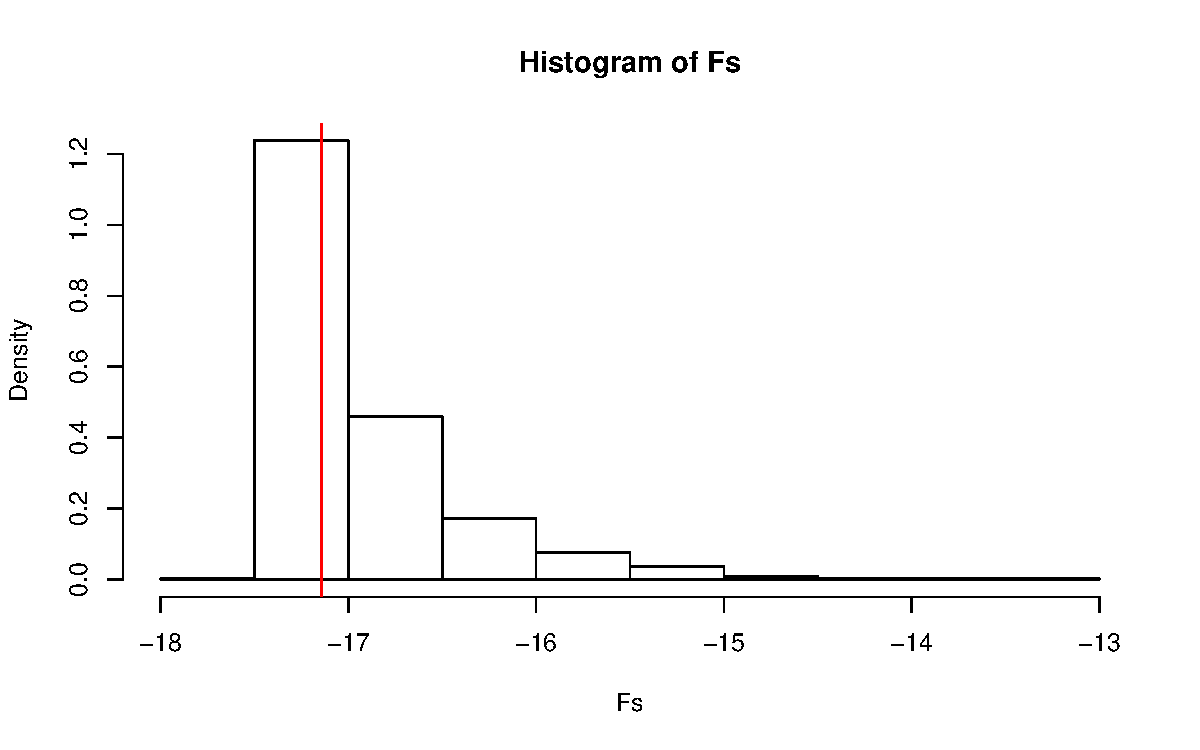
\includegraphics{project2_files/figure-latex/unnamed-chunk-4-1} \end{center}

\begin{Shaded}
\begin{Highlighting}[]
\KeywordTok{mean}\NormalTok{(Fs}\OperatorTok{>}\NormalTok{F_obs)}
\end{Highlighting}
\end{Shaded}

\begin{verbatim}
## [1] 0.507
\end{verbatim}

Null hypothesis is there is no difference in the mean distance or spread
between groups. The alternative hypothesis is that there is a difference
in mean distance or spread between groups.The pvalue is very large and
so we would fail to reject the null hypothesis.

\begin{Shaded}
\begin{Highlighting}[]
\CommentTok{#Question 3.}
\NormalTok{rating_c <-}\StringTok{ }\NormalTok{cer}\OperatorTok{$}\NormalTok{rating }\OperatorTok{-}\StringTok{ }\KeywordTok{mean}\NormalTok{(cer}\OperatorTok{$}\NormalTok{rating)}
\NormalTok{sugars_c <-}\StringTok{ }\NormalTok{cer}\OperatorTok{$}\NormalTok{sugars }\OperatorTok{-}\StringTok{ }\KeywordTok{mean}\NormalTok{(cer}\OperatorTok{$}\NormalTok{sugars)}
\NormalTok{calories_c<-}\StringTok{ }\NormalTok{cer}\OperatorTok{$}\NormalTok{calories }\OperatorTok{-}\StringTok{ }\KeywordTok{mean}\NormalTok{(cer}\OperatorTok{$}\NormalTok{calories)}
\NormalTok{sodium_c<-}\StringTok{ }\NormalTok{cer}\OperatorTok{$}\NormalTok{sodium }\OperatorTok{-}\StringTok{ }\KeywordTok{mean}\NormalTok{(cer}\OperatorTok{$}\NormalTok{sodium)}


\CommentTok{#linear regresssion}
\NormalTok{fit<-}\StringTok{ }\KeywordTok{lm}\NormalTok{(rating}\OperatorTok{~}\NormalTok{calories_c}\OperatorTok{*}\NormalTok{shelf, }\DataTypeTok{data =}\NormalTok{ cer)}
\KeywordTok{summary}\NormalTok{(fit)}
\end{Highlighting}
\end{Shaded}

\begin{verbatim}
## 
## Call:
## lm(formula = rating ~ calories_c * shelf, data = cer)
## 
## Residuals:
##     Min      1Q  Median      3Q     Max 
## -13.730  -6.198  -1.145   4.365  25.476 
## 
## Coefficients:
##                        Estimate Std. Error t value Pr(>|t|)    
## (Intercept)             41.1711     2.0449  20.134  < 2e-16 ***
## calories_c              -1.1349     0.2066  -5.493 5.81e-07 ***
## shelfMiddle             -2.5714     2.7830  -0.924 0.358626    
## shelfTop                 4.4053     2.4599   1.791 0.077588 .  
## calories_c:shelfMiddle  -0.2385     0.3076  -0.776 0.440574    
## calories_c:shelfTop      0.7367     0.2129   3.460 0.000918 ***
## ---
## Signif. codes:  0 '***' 0.001 '**' 0.01 '*' 0.05 '.' 0.1 ' ' 1
## 
## Residual standard error: 8.199 on 71 degrees of freedom
## Multiple R-squared:  0.6817, Adjusted R-squared:  0.6593 
## F-statistic: 30.41 on 5 and 71 DF,  p-value: < 2.2e-16
\end{verbatim}

\begin{Shaded}
\begin{Highlighting}[]
\CommentTok{#linear regression plot}
\KeywordTok{qplot}\NormalTok{(}\DataTypeTok{x =}\NormalTok{ calories, }\DataTypeTok{y =}\NormalTok{ rating, }\DataTypeTok{color =}\NormalTok{ shelf, }\DataTypeTok{data =}\NormalTok{ cer) }\OperatorTok{+}
\KeywordTok{stat_smooth}\NormalTok{(}\DataTypeTok{method =} \StringTok{"lm"}\NormalTok{, }\DataTypeTok{se =} \OtherTok{FALSE}\NormalTok{, }\DataTypeTok{fullrange =} \OtherTok{TRUE}\NormalTok{)}
\end{Highlighting}
\end{Shaded}

\begin{center}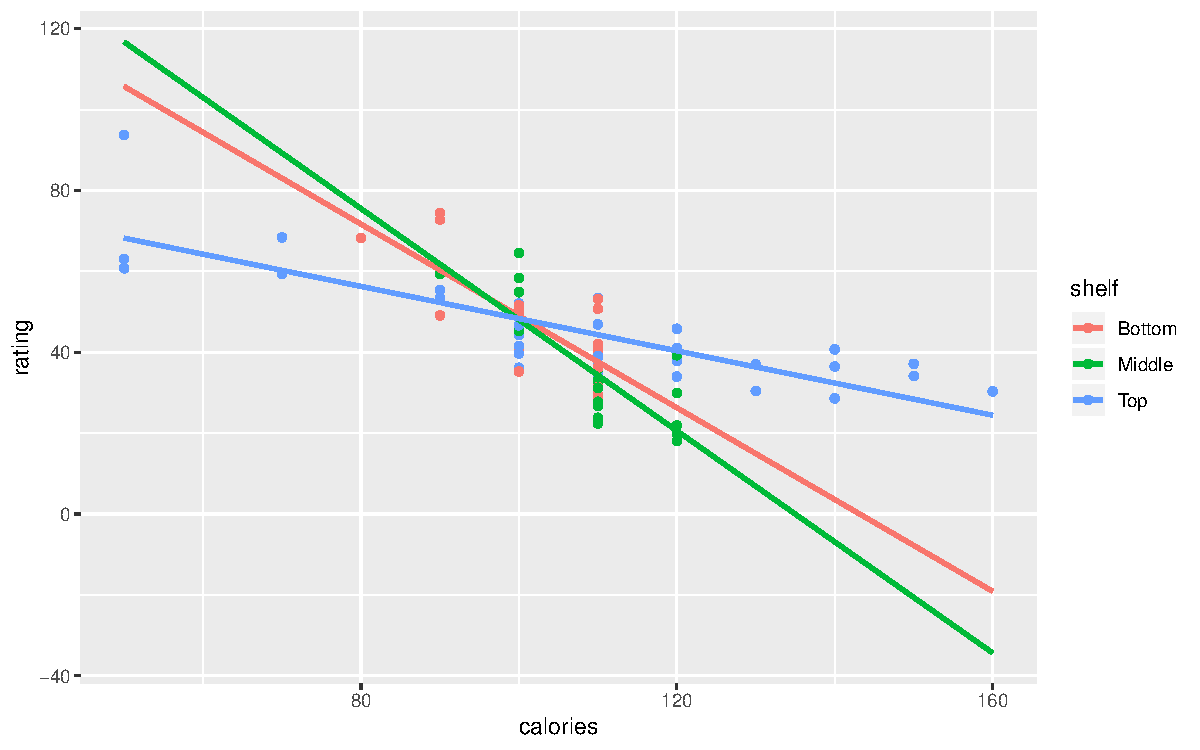
\includegraphics{project2_files/figure-latex/unnamed-chunk-5-1} \end{center}

\begin{Shaded}
\begin{Highlighting}[]
\CommentTok{#checking assumptions}
\NormalTok{resids<-fit}\OperatorTok{$}\NormalTok{residuals; fitvals<-fit}\OperatorTok{$}\NormalTok{fitted.values}
\KeywordTok{ggplot}\NormalTok{()}\OperatorTok{+}\KeywordTok{geom_point}\NormalTok{(}\KeywordTok{aes}\NormalTok{(fitvals,resids))}\OperatorTok{+}\KeywordTok{geom_hline}\NormalTok{(}\DataTypeTok{yintercept=}\DecValTok{0}\NormalTok{, }\DataTypeTok{col=}\StringTok{"red"}\NormalTok{) }\CommentTok{#checks for linearity and homoskedacity}
\end{Highlighting}
\end{Shaded}

\begin{center}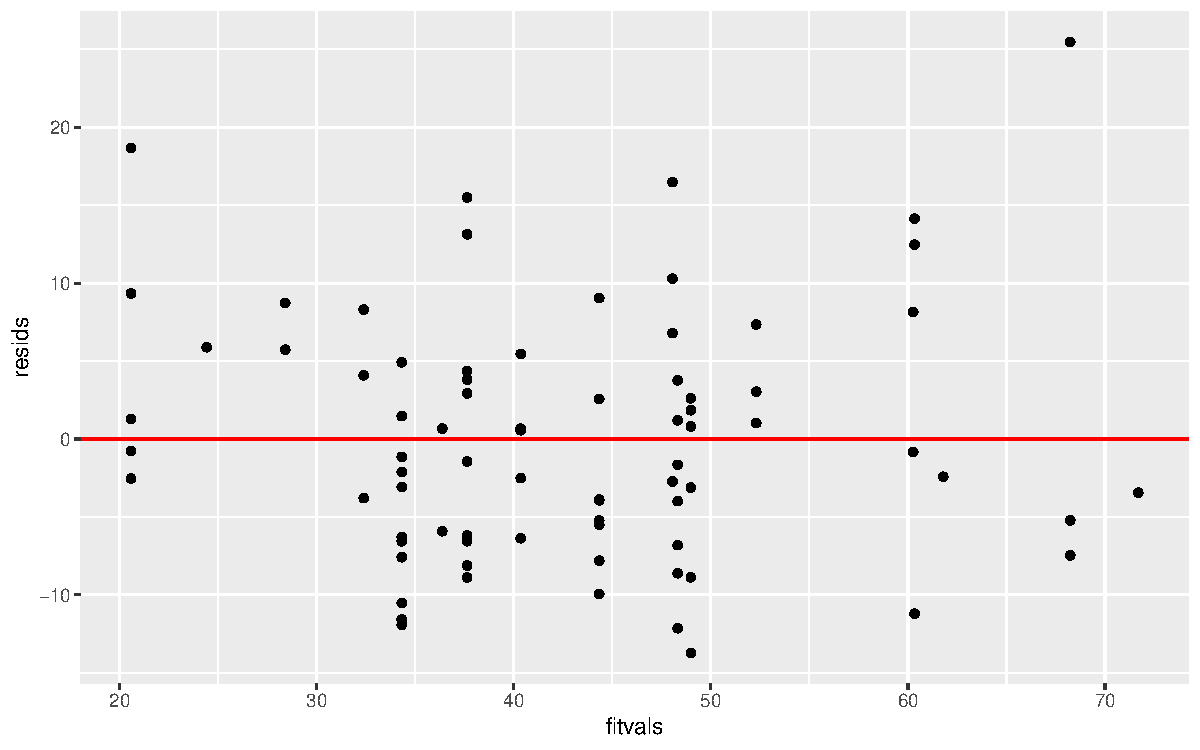
\includegraphics{project2_files/figure-latex/unnamed-chunk-5-2} \end{center}

\begin{Shaded}
\begin{Highlighting}[]
\KeywordTok{ggplot}\NormalTok{()}\OperatorTok{+}\KeywordTok{geom_histogram}\NormalTok{(}\KeywordTok{aes}\NormalTok{(resids),}\DataTypeTok{bins=}\DecValTok{20}\NormalTok{) }\CommentTok{#normality}
\end{Highlighting}
\end{Shaded}

\begin{center}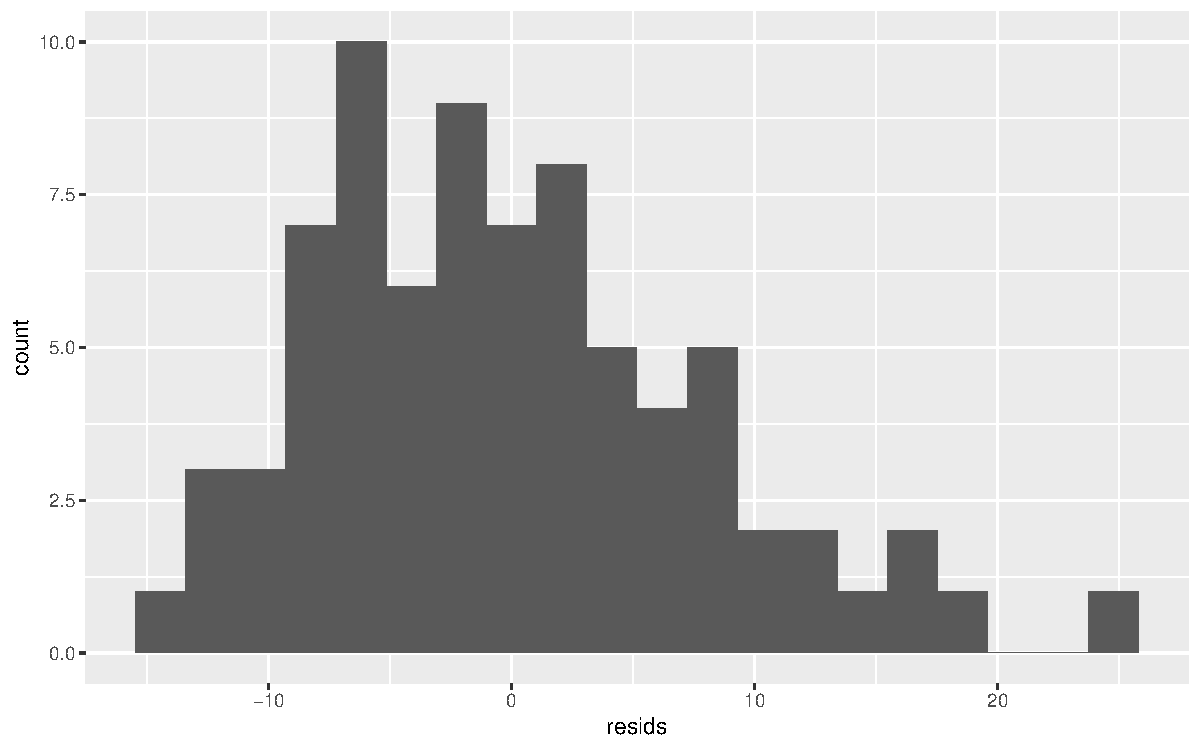
\includegraphics{project2_files/figure-latex/unnamed-chunk-5-3} \end{center}

\begin{Shaded}
\begin{Highlighting}[]
\KeywordTok{ggplot}\NormalTok{()}\OperatorTok{+}\KeywordTok{geom_qq}\NormalTok{(}\KeywordTok{aes}\NormalTok{(}\DataTypeTok{sample=}\NormalTok{resids))}\OperatorTok{+}\KeywordTok{geom_qq_line}\NormalTok{(}\KeywordTok{aes}\NormalTok{(}\DataTypeTok{sample=}\NormalTok{resids), }\DataTypeTok{color=}\StringTok{'red'}\NormalTok{) }\CommentTok{#normality}
\end{Highlighting}
\end{Shaded}

\begin{center}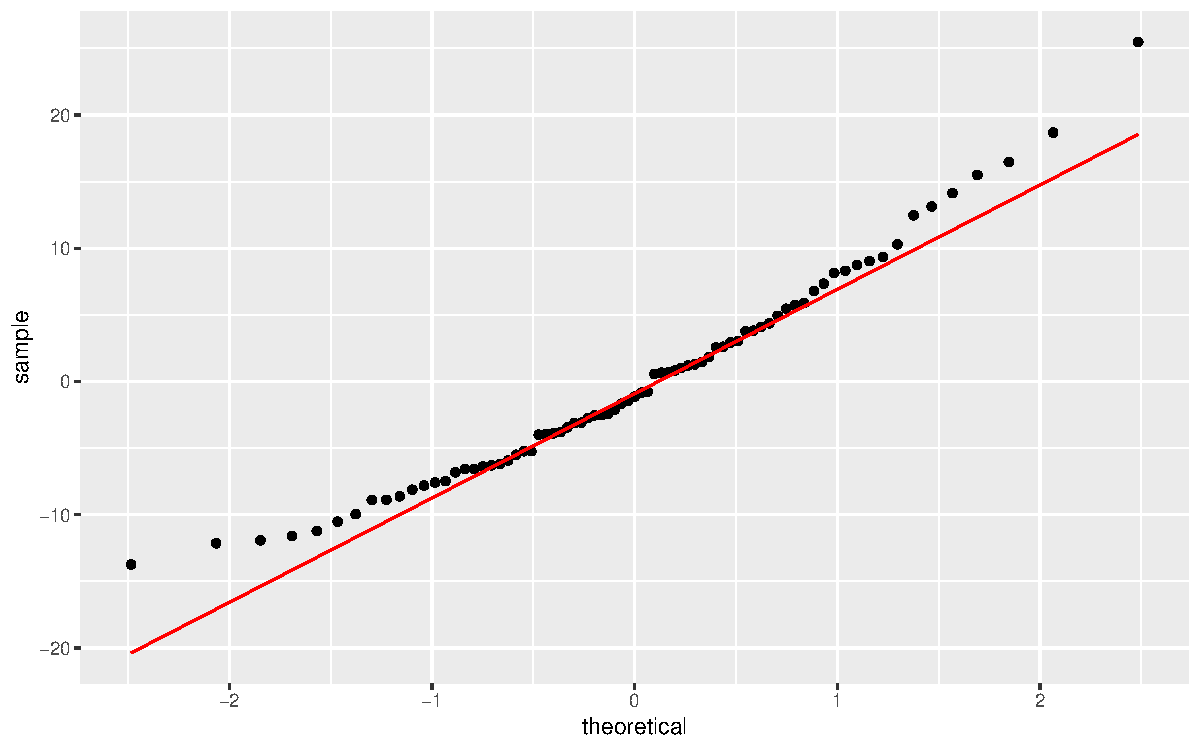
\includegraphics{project2_files/figure-latex/unnamed-chunk-5-4} \end{center}

\begin{Shaded}
\begin{Highlighting}[]
\CommentTok{#regression results}
\KeywordTok{coeftest}\NormalTok{(fit, }\DataTypeTok{vcov. =} \KeywordTok{vcovHC}\NormalTok{(fit))}
\end{Highlighting}
\end{Shaded}

\begin{verbatim}
## 
## t test of coefficients:
## 
##                        Estimate Std. Error t value  Pr(>|t|)    
## (Intercept)            41.17107    2.20473 18.6740 < 2.2e-16 ***
## calories_c             -1.13489    0.25952 -4.3731 4.115e-05 ***
## shelfMiddle            -2.57143    3.03737 -0.8466  0.400063    
## shelfTop                4.40525    2.59364  1.6985  0.093795 .  
## calories_c:shelfMiddle -0.23854    0.37296 -0.6396  0.524507    
## calories_c:shelfTop     0.73666    0.27155  2.7128  0.008365 ** 
## ---
## Signif. codes:  0 '***' 0.001 '**' 0.01 '*' 0.05 '.' 0.1 ' ' 1
\end{verbatim}

\begin{quote}
\begin{itemize}
\tightlist
\item
  Intercept: Predicted rating for a cereal with calories kept constant
  controlling for shelf placement is 41.17 points.
\item
  ShelfMiddle: Controlling for calories, rating for the middle shelf
  group is 2.57 points lower than the bottom shelf on average.
\item
  ShelfTop: Controlling for calories, rating for the top shelf group is
  4.4 points higher than the bottom shelf on average.
\item
  calories\_c: There is a decrease of -1.13 rating points for every one
  unit increase in sugar on average.
\item
  shelfMiddle:calories\_c: The slope for calories on rating is .239
  times lower for the middle shelf compared to the bottom shelf.
\item
  shelfTop:calories\_c: The slope for calories on rating is .737 times
  higher for the top shelf compared to the bottom shelf.
\end{itemize}
\end{quote}

\begin{quote}
\begin{itemize}
\tightlist
\item
  The original standard errors were 2.78 and 2.46 for the middle and top
  shelves while the interaction and rating were all around .2. The
  significant p values were for calories and top shelf. The robust
  standard errors increased for the middle shelf and slightly decreased
  for the top shelf but the interaction between top shelf and calories
  was now significant.
\end{itemize}
\end{quote}

\begin{quote}
\begin{itemize}
\tightlist
\item
  Based on the adjusted r-squared value of the original model, we can
  estimate that rating and shelf level can explain about 65\% of the
  variance in sugar per serving of cereal.
\end{itemize}
\end{quote}

\begin{Shaded}
\begin{Highlighting}[]
\CommentTok{#Question 4}
\CommentTok{#bootstrap SE}

\NormalTok{samp_distn<-}\KeywordTok{replicate}\NormalTok{(}\DecValTok{5000}\NormalTok{, \{}
\NormalTok{boot_dat <-}\StringTok{ }\KeywordTok{sample_frac}\NormalTok{(cer, }\DataTypeTok{replace=}\NormalTok{T) }\CommentTok{#bootstrap your data}
\NormalTok{fit <-}\StringTok{ }\KeywordTok{lm}\NormalTok{(rating}\OperatorTok{~}\NormalTok{calories_c}\OperatorTok{*}\NormalTok{shelf, }\DataTypeTok{data=}\NormalTok{boot_dat) }\CommentTok{#fit model}
\KeywordTok{coef}\NormalTok{(fit) }\CommentTok{#save coefs}
\NormalTok{\})}
\CommentTok{## Estimated SEs}
\NormalTok{samp_distn }\OperatorTok\StringTok{ }\NormalTok{t }\OperatorTok\StringTok{ }\NormalTok{as.data.frame }\OperatorTok\StringTok{ }\KeywordTok{summarize_all}\NormalTok{(sd)}
\end{Highlighting}
\end{Shaded}

\begin{verbatim}
##   (Intercept) calories_c shelfMiddle shelfTop calories_c:shelfMiddle calories_c:shelfTop
## 1    3.118898  0.1802748    4.425616 3.756992              0.2524729           0.2171494
\end{verbatim}

After running bootstrap errors, the middle and top shelf increased in
value compared to the original as well as the robust errors. The
calories st. error got smaller. The interaction between calories and
middle shelf and top shelf decreased but only slightly. Since the SEs
for shelves got bigger, we can assume that the p values also got bigger
for those variables.

\begin{Shaded}
\begin{Highlighting}[]
\CommentTok{#Question 5}
\KeywordTok{head}\NormalTok{(cer)}
\end{Highlighting}
\end{Shaded}

\begin{verbatim}
## # A tibble: 6 x 6
##   name                      mfr   calories sodium shelf  rating
##   <chr>                     <fct>    <dbl>  <dbl> <fct>   <dbl>
## 1 100% Bran                 0           70    130 Top      68.4
## 2 100% Natural Bran         0          120     15 Top      34.0
## 3 All-Bran                  1           70    260 Top      59.4
## 4 All-Bran with Extra Fiber 1           50    140 Top      93.7
## 5 Almond Delight            0          110    200 Top      34.4
## 6 Apple Cinnamon Cheerios   0          110    180 Bottom   29.5
\end{verbatim}

\begin{Shaded}
\begin{Highlighting}[]
\NormalTok{fit3<-}\StringTok{ }\KeywordTok{glm}\NormalTok{(mfr}\OperatorTok{~}\NormalTok{sodium}\OperatorTok{+}\NormalTok{rating, }\DataTypeTok{data =}\NormalTok{ cer, }\DataTypeTok{family=}\KeywordTok{binomial}\NormalTok{(}\DataTypeTok{link=}\StringTok{"logit"}\NormalTok{))}
\KeywordTok{coeftest}\NormalTok{(fit3)}
\end{Highlighting}
\end{Shaded}

\begin{verbatim}
## 
## z test of coefficients:
## 
##               Estimate Std. Error z value Pr(>|z|)  
## (Intercept) -2.4829901  1.2114207 -2.0497   0.0404 *
## sodium       0.0045534  0.0033596  1.3553   0.1753  
## rating       0.0205273  0.0195455  1.0502   0.2936  
## ---
## Signif. codes:  0 '***' 0.001 '**' 0.01 '*' 0.05 '.' 0.1 ' ' 1
\end{verbatim}

\begin{Shaded}
\begin{Highlighting}[]
\KeywordTok{exp}\NormalTok{(}\KeywordTok{coef}\NormalTok{(fit3))}
\end{Highlighting}
\end{Shaded}

\begin{verbatim}
## (Intercept)      sodium      rating 
##   0.0834932   1.0045637   1.0207395
\end{verbatim}

\begin{Shaded}
\begin{Highlighting}[]
\NormalTok{prob<-}\StringTok{ }\KeywordTok{predict}\NormalTok{(fit3, }\DataTypeTok{type =} \StringTok{"response"}\NormalTok{)}

\CommentTok{#confusion matrix}
\KeywordTok{table}\NormalTok{(}\DataTypeTok{predict=}\KeywordTok{as.numeric}\NormalTok{(prob}\OperatorTok{>}\NormalTok{.}\DecValTok{5}\NormalTok{),}\DataTypeTok{truth=}\NormalTok{cer}\OperatorTok{$}\NormalTok{mfr)}\OperatorTok\NormalTok{addmargins}
\end{Highlighting}
\end{Shaded}

\begin{verbatim}
##        truth
## predict  0  1 Sum
##     0   54 22  76
##     1    0  1   1
##     Sum 54 23  77
\end{verbatim}

\begin{Shaded}
\begin{Highlighting}[]
\CommentTok{#accuracy}
\NormalTok{(}\DecValTok{54}\OperatorTok{+}\DecValTok{1}\NormalTok{)}\OperatorTok{/}\DecValTok{77}
\end{Highlighting}
\end{Shaded}

\begin{verbatim}
## [1] 0.7142857
\end{verbatim}

\begin{Shaded}
\begin{Highlighting}[]
\CommentTok{#sensitivity}
\NormalTok{(}\DecValTok{1}\OperatorTok{/}\DecValTok{23}\NormalTok{)}
\end{Highlighting}
\end{Shaded}

\begin{verbatim}
## [1] 0.04347826
\end{verbatim}

\begin{Shaded}
\begin{Highlighting}[]
\CommentTok{#specificity}
\DecValTok{54}\OperatorTok{/}\DecValTok{54}
\end{Highlighting}
\end{Shaded}

\begin{verbatim}
## [1] 1
\end{verbatim}

\begin{Shaded}
\begin{Highlighting}[]
\CommentTok{#ppv}
\DecValTok{1}\OperatorTok{/}\DecValTok{1}
\end{Highlighting}
\end{Shaded}

\begin{verbatim}
## [1] 1
\end{verbatim}

\begin{Shaded}
\begin{Highlighting}[]
\CommentTok{#plot densit of log odds}
\NormalTok{odds<-}\ControlFlowTok{function}\NormalTok{(p)p}\OperatorTok{/}\NormalTok{(}\DecValTok{1}\OperatorTok{-}\NormalTok{p)}
\NormalTok{p<-}\KeywordTok{seq}\NormalTok{(}\DecValTok{0}\NormalTok{,}\DecValTok{1}\NormalTok{,}\DataTypeTok{by=}\NormalTok{.}\DecValTok{1}\NormalTok{)}
\KeywordTok{cbind}\NormalTok{(p, }\DataTypeTok{odds=}\KeywordTok{odds}\NormalTok{(p))}\OperatorTok\KeywordTok{round}\NormalTok{(}\DecValTok{4}\NormalTok{)}
\end{Highlighting}
\end{Shaded}

\begin{verbatim}
##         p   odds
##  [1,] 0.0 0.0000
##  [2,] 0.1 0.1111
##  [3,] 0.2 0.2500
##  [4,] 0.3 0.4286
##  [5,] 0.4 0.6667
##  [6,] 0.5 1.0000
##  [7,] 0.6 1.5000
##  [8,] 0.7 2.3333
##  [9,] 0.8 4.0000
## [10,] 0.9 9.0000
## [11,] 1.0    Inf
\end{verbatim}

\begin{Shaded}
\begin{Highlighting}[]
\NormalTok{logit<-}\ControlFlowTok{function}\NormalTok{(p)}\KeywordTok{log}\NormalTok{(}\KeywordTok{odds}\NormalTok{(p))}
\KeywordTok{cbind}\NormalTok{(p, }\DataTypeTok{odds=}\KeywordTok{odds}\NormalTok{(p),}\DataTypeTok{logit=}\KeywordTok{logit}\NormalTok{(p))}\OperatorTok\KeywordTok{round}\NormalTok{(}\DecValTok{4}\NormalTok{)}
\end{Highlighting}
\end{Shaded}

\begin{verbatim}
##         p   odds   logit
##  [1,] 0.0 0.0000    -Inf
##  [2,] 0.1 0.1111 -2.1972
##  [3,] 0.2 0.2500 -1.3863
##  [4,] 0.3 0.4286 -0.8473
##  [5,] 0.4 0.6667 -0.4055
##  [6,] 0.5 1.0000  0.0000
##  [7,] 0.6 1.5000  0.4055
##  [8,] 0.7 2.3333  0.8473
##  [9,] 0.8 4.0000  1.3863
## [10,] 0.9 9.0000  2.1972
## [11,] 1.0    Inf     Inf
\end{verbatim}

\begin{Shaded}
\begin{Highlighting}[]
\KeywordTok{ggplot}\NormalTok{()}\OperatorTok{+}\KeywordTok{stat_function}\NormalTok{(}\KeywordTok{aes}\NormalTok{(p),}\DataTypeTok{fun=}\NormalTok{logit,}\DataTypeTok{geom=}\StringTok{"line"}\NormalTok{)}\OperatorTok{+}\KeywordTok{ylab}\NormalTok{(}\StringTok{"g(p)=logit(p)"}\NormalTok{)}\OperatorTok{+}\KeywordTok{xlab}\NormalTok{(}\StringTok{"p"}\NormalTok{)}
\end{Highlighting}
\end{Shaded}

\begin{center}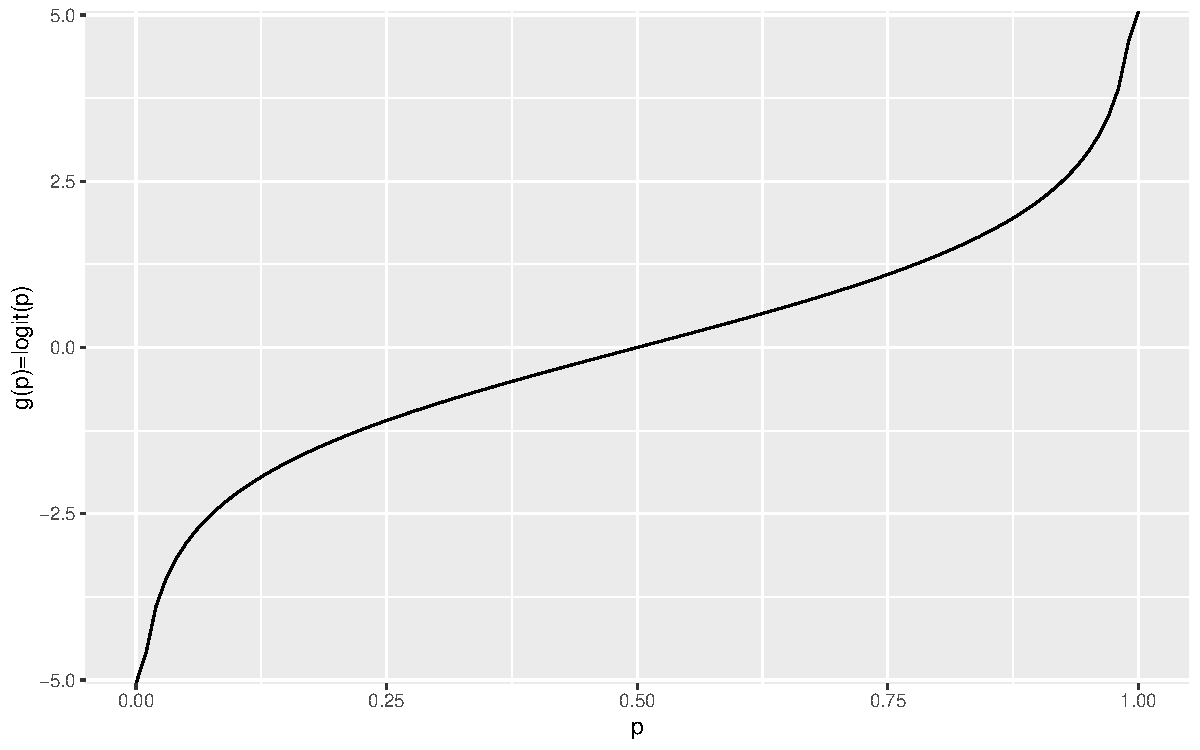
\includegraphics{project2_files/figure-latex/unnamed-chunk-7-1} \end{center}

\begin{quote}
\begin{itemize}
\tightlist
\item
  Intercept: odds of manufacterer being Kellogs when sodium and rating
  are held constant is .083.
\item
  sodium: controlling for rating, for every one mg increase in sodium,
  odds of the manufacterer being Kellogs increase by a factor of 1.0046
\item
  rating: controlling for sodium, for every one unit increase in rating,
  odds of the manufacterer being Kellogs increase by a factor of 1.0207
\end{itemize}
\end{quote}

\begin{Shaded}
\begin{Highlighting}[]
\CommentTok{# ROC curve}
\CommentTok{#install.packages("plotROC")}
\KeywordTok{library}\NormalTok{(plotROC)}

\NormalTok{cer1}\OperatorTok{$}\NormalTok{mfr<-}\StringTok{ }\KeywordTok{as.factor}\NormalTok{(cer1}\OperatorTok{$}\NormalTok{mfr)}

\NormalTok{ROCplot<-}\KeywordTok{ggplot}\NormalTok{(cer1)}\OperatorTok{+}\KeywordTok{geom_roc}\NormalTok{(}\KeywordTok{aes}\NormalTok{(}\DataTypeTok{d=}\NormalTok{mfr,}\DataTypeTok{m=}\NormalTok{prob), }\DataTypeTok{n.cuts=}\DecValTok{0}\NormalTok{)}\OperatorTok{+}
\KeywordTok{geom_segment}\NormalTok{(}\KeywordTok{aes}\NormalTok{(}\DataTypeTok{x=}\DecValTok{0}\NormalTok{,}\DataTypeTok{xend=}\DecValTok{1}\NormalTok{,}\DataTypeTok{y=}\DecValTok{0}\NormalTok{,}\DataTypeTok{yend=}\DecValTok{1}\NormalTok{),}\DataTypeTok{lty=}\DecValTok{2}\NormalTok{)}
\NormalTok{ROCplot}
\end{Highlighting}
\end{Shaded}

\begin{center}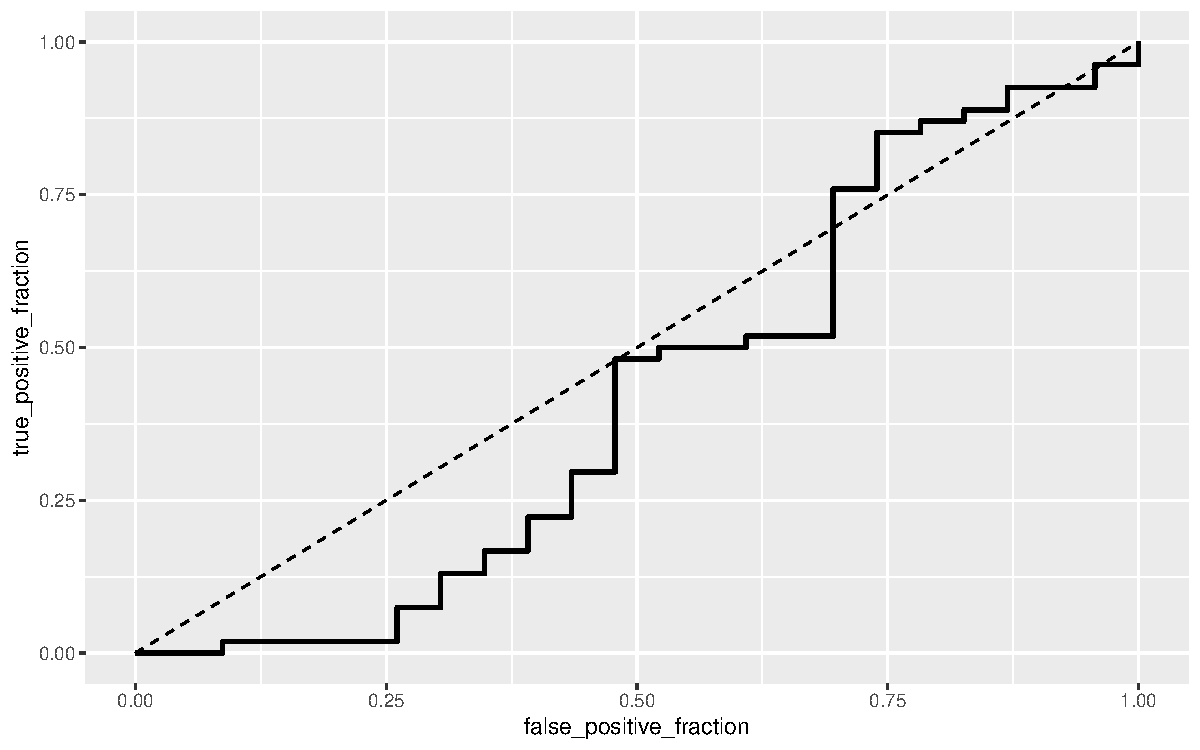
\includegraphics{project2_files/figure-latex/unnamed-chunk-8-1} \end{center}

\begin{Shaded}
\begin{Highlighting}[]
\CommentTok{#AUC}
\KeywordTok{calc_auc}\NormalTok{(ROCplot)}
\end{Highlighting}
\end{Shaded}

\begin{verbatim}
##   PANEL group       AUC
## 1     1    -1 0.4202899
\end{verbatim}

\begin{Shaded}
\begin{Highlighting}[]
\CommentTok{#needed for function}
\NormalTok{class_diag<-}\ControlFlowTok{function}\NormalTok{(probs,truth)\{}
  
\NormalTok{  tab<-}\KeywordTok{table}\NormalTok{(}\KeywordTok{factor}\NormalTok{(probs}\OperatorTok{>}\NormalTok{.}\DecValTok{5}\NormalTok{,}\DataTypeTok{levels=}\KeywordTok{c}\NormalTok{(}\StringTok{"FALSE"}\NormalTok{,}\StringTok{"TRUE"}\NormalTok{)),truth)}
\NormalTok{  acc=}\KeywordTok{sum}\NormalTok{(}\KeywordTok{diag}\NormalTok{(tab))}\OperatorTok{/}\KeywordTok{sum}\NormalTok{(tab)}
\NormalTok{  sens=tab[}\DecValTok{2}\NormalTok{,}\DecValTok{2}\NormalTok{]}\OperatorTok{/}\KeywordTok{colSums}\NormalTok{(tab)[}\DecValTok{2}\NormalTok{]}
\NormalTok{  spec=tab[}\DecValTok{1}\NormalTok{,}\DecValTok{1}\NormalTok{]}\OperatorTok{/}\KeywordTok{colSums}\NormalTok{(tab)[}\DecValTok{1}\NormalTok{]}
\NormalTok{  ppv=tab[}\DecValTok{2}\NormalTok{,}\DecValTok{2}\NormalTok{]}\OperatorTok{/}\KeywordTok{rowSums}\NormalTok{(tab)[}\DecValTok{2}\NormalTok{]}

  \ControlFlowTok{if}\NormalTok{(}\KeywordTok{is.numeric}\NormalTok{(truth)}\OperatorTok{==}\OtherTok{FALSE} \OperatorTok{&}\StringTok{ }\KeywordTok{is.logical}\NormalTok{(truth)}\OperatorTok{==}\OtherTok{FALSE}\NormalTok{) truth<-}\KeywordTok{as.numeric}\NormalTok{(truth)}\OperatorTok{-}\DecValTok{1}
  
  \CommentTok{#CALCULATE EXACT AUC}
\NormalTok{  ord<-}\KeywordTok{order}\NormalTok{(probs, }\DataTypeTok{decreasing=}\OtherTok{TRUE}\NormalTok{)}
\NormalTok{  probs <-}\StringTok{ }\NormalTok{probs[ord]; truth <-}\StringTok{ }\NormalTok{truth[ord]}
  
\NormalTok{  TPR=}\KeywordTok{cumsum}\NormalTok{(truth)}\OperatorTok{/}\KeywordTok{max}\NormalTok{(}\DecValTok{1}\NormalTok{,}\KeywordTok{sum}\NormalTok{(truth)) }
\NormalTok{  FPR=}\KeywordTok{cumsum}\NormalTok{(}\OperatorTok{!}\NormalTok{truth)}\OperatorTok{/}\KeywordTok{max}\NormalTok{(}\DecValTok{1}\NormalTok{,}\KeywordTok{sum}\NormalTok{(}\OperatorTok{!}\NormalTok{truth))}
  
\NormalTok{  dup<-}\KeywordTok{c}\NormalTok{(probs[}\OperatorTok{-}\DecValTok{1}\NormalTok{]}\OperatorTok{>=}\NormalTok{probs[}\OperatorTok{-}\KeywordTok{length}\NormalTok{(probs)], }\OtherTok{FALSE}\NormalTok{)}
\NormalTok{  TPR<-}\KeywordTok{c}\NormalTok{(}\DecValTok{0}\NormalTok{,TPR[}\OperatorTok{!}\NormalTok{dup],}\DecValTok{1}\NormalTok{); FPR<-}\KeywordTok{c}\NormalTok{(}\DecValTok{0}\NormalTok{,FPR[}\OperatorTok{!}\NormalTok{dup],}\DecValTok{1}\NormalTok{)}
  
\NormalTok{  n <-}\StringTok{ }\KeywordTok{length}\NormalTok{(TPR)}
\NormalTok{  auc<-}\StringTok{ }\KeywordTok{sum}\NormalTok{( ((TPR[}\OperatorTok{-}\DecValTok{1}\NormalTok{]}\OperatorTok{+}\NormalTok{TPR[}\OperatorTok{-}\NormalTok{n])}\OperatorTok{/}\DecValTok{2}\NormalTok{) }\OperatorTok{*}\StringTok{ }\NormalTok{(FPR[}\OperatorTok{-}\DecValTok{1}\NormalTok{]}\OperatorTok{-}\NormalTok{FPR[}\OperatorTok{-}\NormalTok{n]) )}

  \KeywordTok{data.frame}\NormalTok{(acc,sens,spec,ppv,auc)}
\NormalTok{\}}
\end{Highlighting}
\end{Shaded}

\begin{Shaded}
\begin{Highlighting}[]
\CommentTok{#Question 5 continued}

\KeywordTok{set.seed}\NormalTok{(}\DecValTok{1234}\NormalTok{)}
\NormalTok{k=}\DecValTok{10} \CommentTok{#choose number of folds}
\NormalTok{data<-cer[}\KeywordTok{sample}\NormalTok{(}\KeywordTok{nrow}\NormalTok{(cer)),] }\CommentTok{#randomly order rows}
\NormalTok{folds<-}\KeywordTok{cut}\NormalTok{(}\KeywordTok{seq}\NormalTok{(}\DecValTok{1}\OperatorTok{:}\KeywordTok{nrow}\NormalTok{(cer)),}\DataTypeTok{breaks=}\NormalTok{k,}\DataTypeTok{labels=}\NormalTok{F) }\CommentTok{#create folds}
\NormalTok{diags<-}\OtherTok{NULL}
\ControlFlowTok{for}\NormalTok{(i }\ControlFlowTok{in} \DecValTok{1}\OperatorTok{:}\NormalTok{k)\{}
\CommentTok{## Create training and test sets}
\NormalTok{train<-data[folds}\OperatorTok{!=}\NormalTok{i,]}
\NormalTok{test<-data[folds}\OperatorTok{==}\NormalTok{i,]}
\NormalTok{truth<-test}\OperatorTok{$}\NormalTok{mfr }\CommentTok{## Truth labels for fold i}
\CommentTok{## Train model on training set (all but fold i)}
\NormalTok{fit<-}\KeywordTok{glm}\NormalTok{(mfr}\OperatorTok{~}\NormalTok{rating}\OperatorTok{+}\NormalTok{sodium,}\DataTypeTok{data=}\NormalTok{train,}\DataTypeTok{family=}\StringTok{"binomial"}\NormalTok{)}
\CommentTok{## Test model on test set (fold i)}
\NormalTok{probs<-}\KeywordTok{predict}\NormalTok{(fit,}\DataTypeTok{newdata =}\NormalTok{ test,}\DataTypeTok{type=}\StringTok{"response"}\NormalTok{)}
\CommentTok{## Get diagnostics for fold i}
\NormalTok{diags<-}\KeywordTok{rbind}\NormalTok{(diags,}\KeywordTok{class_diag}\NormalTok{(probs,truth))}
\NormalTok{\}}
\KeywordTok{summarize_all}\NormalTok{(diags,mean)}
\end{Highlighting}
\end{Shaded}

\begin{verbatim}
##         acc sens      spec ppv       auc
## 1 0.6821429    0 0.9833333 NaN 0.5257143
\end{verbatim}

\begin{quote}
\begin{itemize}
\tightlist
\item
  The AUC is .45 which would fall below the Bad category.
\item
  The out of sample performance for accuracy is .69, the specificity is
  .98, and the AUC is .45.
\end{itemize}
\end{quote}

\begin{Shaded}
\begin{Highlighting}[]
\CommentTok{#Question 6}

\CommentTok{#LASSO}
\CommentTok{#install.packages("glmnet")}
\KeywordTok{library}\NormalTok{(glmnet)}
\CommentTok{#install.packages("plyr")}
\KeywordTok{library}\NormalTok{(dplyr)}

\NormalTok{y<-}\KeywordTok{as.matrix}\NormalTok{(cer1}\OperatorTok{$}\NormalTok{mfr) }\CommentTok{#grab response}
\NormalTok{x<-}\KeywordTok{model.matrix}\NormalTok{(mfr}\OperatorTok{~}\NormalTok{.,}\DataTypeTok{data=}\NormalTok{cer1)[,}\OperatorTok{-}\DecValTok{1}\NormalTok{] }\CommentTok{#grab predictors}
\KeywordTok{head}\NormalTok{(x)}
\end{Highlighting}
\end{Shaded}

\begin{verbatim}
##   calories sodium shelfMiddle shelfTop   rating
## 1       70    130           0        1 68.40297
## 2      120     15           0        1 33.98368
## 3       70    260           0        1 59.42551
## 4       50    140           0        1 93.70491
## 5      110    200           0        1 34.38484
## 6      110    180           0        0 29.50954
\end{verbatim}

\begin{Shaded}
\begin{Highlighting}[]
\NormalTok{cv<-}\KeywordTok{cv.glmnet}\NormalTok{(x,y, }\DataTypeTok{family =} \StringTok{"binomial"}\NormalTok{)}
\NormalTok{lasso<-}\KeywordTok{glmnet}\NormalTok{(x,y,}\DataTypeTok{family =} \StringTok{"binomial"}\NormalTok{, }\DataTypeTok{lambda=}\NormalTok{cv}\OperatorTok{$}\NormalTok{lambda}\FloatTok{.1}\NormalTok{se)}
\KeywordTok{coef}\NormalTok{(lasso)}
\end{Highlighting}
\end{Shaded}

\begin{verbatim}
## 6 x 1 sparse Matrix of class "dgCMatrix"
##                        s0
## (Intercept)  8.534898e-01
## calories     .           
## sodium      -1.590880e-18
## shelfMiddle  .           
## shelfTop     .           
## rating       .
\end{verbatim}

\begin{Shaded}
\begin{Highlighting}[]
\KeywordTok{set.seed}\NormalTok{(}\DecValTok{1234}\NormalTok{)}
\NormalTok{k=}\DecValTok{10} \CommentTok{#choose number of folds}

\NormalTok{data<-cer[}\KeywordTok{sample}\NormalTok{(}\KeywordTok{nrow}\NormalTok{(cer)),] }\CommentTok{#randomly order rows}
\NormalTok{folds<-}\KeywordTok{cut}\NormalTok{(}\KeywordTok{seq}\NormalTok{(}\DecValTok{1}\OperatorTok{:}\KeywordTok{nrow}\NormalTok{(cer)),}\DataTypeTok{breaks=}\NormalTok{k,}\DataTypeTok{labels=}\NormalTok{F) }\CommentTok{#create folds}

\NormalTok{diags<-}\OtherTok{NULL}
\ControlFlowTok{for}\NormalTok{(i }\ControlFlowTok{in} \DecValTok{1}\OperatorTok{:}\NormalTok{k)\{}
  \CommentTok{## Create training and test sets}
\NormalTok{  train<-data[folds}\OperatorTok{!=}\NormalTok{i,] }
\NormalTok{  test<-data[folds}\OperatorTok{==}\NormalTok{i,]}
  
\NormalTok{  truth<-test}\OperatorTok{$}\NormalTok{mfr }\CommentTok{## Truth labels for fold i}
  
  \CommentTok{## Train model on training set (all but fold i)}
\NormalTok{  fit<-}\KeywordTok{glm}\NormalTok{(mfr}\OperatorTok{~}\NormalTok{sodium,}\DataTypeTok{data=}\NormalTok{train,}\DataTypeTok{family=}\StringTok{"binomial"}\NormalTok{)}
  
  \CommentTok{## Test model on test set (fold i) }
\NormalTok{  probs<-}\KeywordTok{predict}\NormalTok{(fit,}\DataTypeTok{newdata =}\NormalTok{ test,}\DataTypeTok{type=}\StringTok{"response"}\NormalTok{)}
  
  \CommentTok{## Get diagnostics for fold i}
\NormalTok{  diags<-}\KeywordTok{rbind}\NormalTok{(diags,}\KeywordTok{class_diag}\NormalTok{(probs,truth))}
\NormalTok{\}}


\KeywordTok{summarize_all}\NormalTok{(diags,mean)}
\end{Highlighting}
\end{Shaded}

\begin{verbatim}
##         acc sens spec ppv       auc
## 1 0.6946429    0    1 NaN 0.5385714
\end{verbatim}

The only variable that was retained was the sodium variable. The AUC for
question 5 was .45 and the out of sample performance was better as the
AUC was .48 and the accuracy went from from .69 to .701. Since these
values are higher, we do not assume overfitting. Add a new chunk by
clicking the \emph{Insert Chunk} button on the toolbar or by pressing
\emph{Cmd+Option+I}.

When you save the notebook, an HTML file containing the code and output
will be saved alongside it (click the \emph{Preview} button or press
\emph{Cmd+Shift+K} to preview the HTML file).

The preview shows you a rendered HTML copy of the contents of the
editor. Consequently, unlike \emph{Knit}, \emph{Preview} does not run
any R code chunks. Instead, the output of the chunk when it was last run
in the editor is displayed.

\end{document}
